\section{Reachability Avoidance}
According to (cite craig) a necessary condition for a solution to exist, is to verify whether it exists in the workspace of the manipulator. Workspace is defined as the end effector's reachable volume(cite craig). Therefore it goes without saying that to ensure that the generated weld paths are valid, we have to ensure that they are free from unreachable points. In the existing system(cite ppr) the robot could only check whether a point lay in the reachable workspace or not, but there was no method to avoid it or generate an alternate path. The only solution was to manually move the work piece to a position, where unreachable points were not present. Manually moving the workpiece created the following problems:
\begin{itemize}
	\item After moving the workpiece, it was necessary to remeasure its position coordinates and enter the new values to the software. Often re measurement was required to ensure that the workpiece has been placed in the proper position.
	\item If more than one edge of a workpiece was needed to welded, and one of the edges fell in a non-reachable position, moving the workpiece and trying to recalibrate its position proved to be an extremely tedious and inefficient method. Often this resulted in abandoning the generated plan and starting anew.
	\item Placing the workpiece in a fixed position on the table every time, provided a sub-optima solution. However this meant that it was necessary to mark positions for each and every workpiece and accurately set them up each and every time they were to be welded.	
\end{itemize} 

Using the 2Dof rotary table to solve the problem of reachability provided the following advantages:
\begin{itemize}
	\item The table can be moved multiple times and each and every time we will know the precise position of the workpiece using algorithm (\ref{algo2}).
	\item Since we also calculate the new position of the weld path, when the table is rotated,(using algorithm (\ref{algo3}) ), hence we can generate weld paths for different edges, without manually altering the workpiece position.
	\item Constraint on placing the workpiece at a fixed position is removed, thus providing greater flexibility to the welding process.
\end{itemize}
\subsection{Reachability and Motion Planning}
In (ppr paper), an inverse kinematic based approach for detecting whether a point is unreachable or not is implemented. It takes the Cartesian coordinates of a point and computes the Inverse Kinematics to get the joint values. If the solution generated is valid, then the point is flagged as reachable, otherwise it is marked as unreachable. In order to generate valid plan paths with the motion planner, it was necessary to link the reachability checker with the planning algorithm. 
The steps for detecting unreachable points with the motion planner are described below:
\begin{itemize}
	\item After the path to be weld has been defined, the start and goal points of the selected edge are used to create the OMPL space, using the methodology described in (ppr).
	\item The planner(in our case RRTstar) is configured and planning is started.
	\item OMPL uses a state validity checker class to check whether a generated sample is valid or not. The definition of validity can be set by the user. In our case we link the reachability detection algorithm with the validity checker.
	\item The planner returns a true or false value based on whether a point is reachable or not.
	\item If all the planner is successfully able to connect the start and goal points without having any invalid points in between, the solution is marked as successful and the cumulative cost value of the path is calculated using equation(\ref{eq25}).
	\item If however the planner fails to find a valid solution, we assign a very high cost value to the failed solution. 
\end{itemize} 

\subsection{Use Case Description}
\label{ssec:usc1}
We present a use case, figure(\ref{fig:rc1}), the  workpiece edge to be welded is marked with yellow. We generate the following plots \ref{fig:rc1} and \ref{fig:rc2} for visualizing the cost surface and the reachable planned paths for
 the manipulator with respect to the movement of the workpiece.
\begin{figure}[!ht] %  figure placement: here, top, bottom, or page
	\centering
	\frame{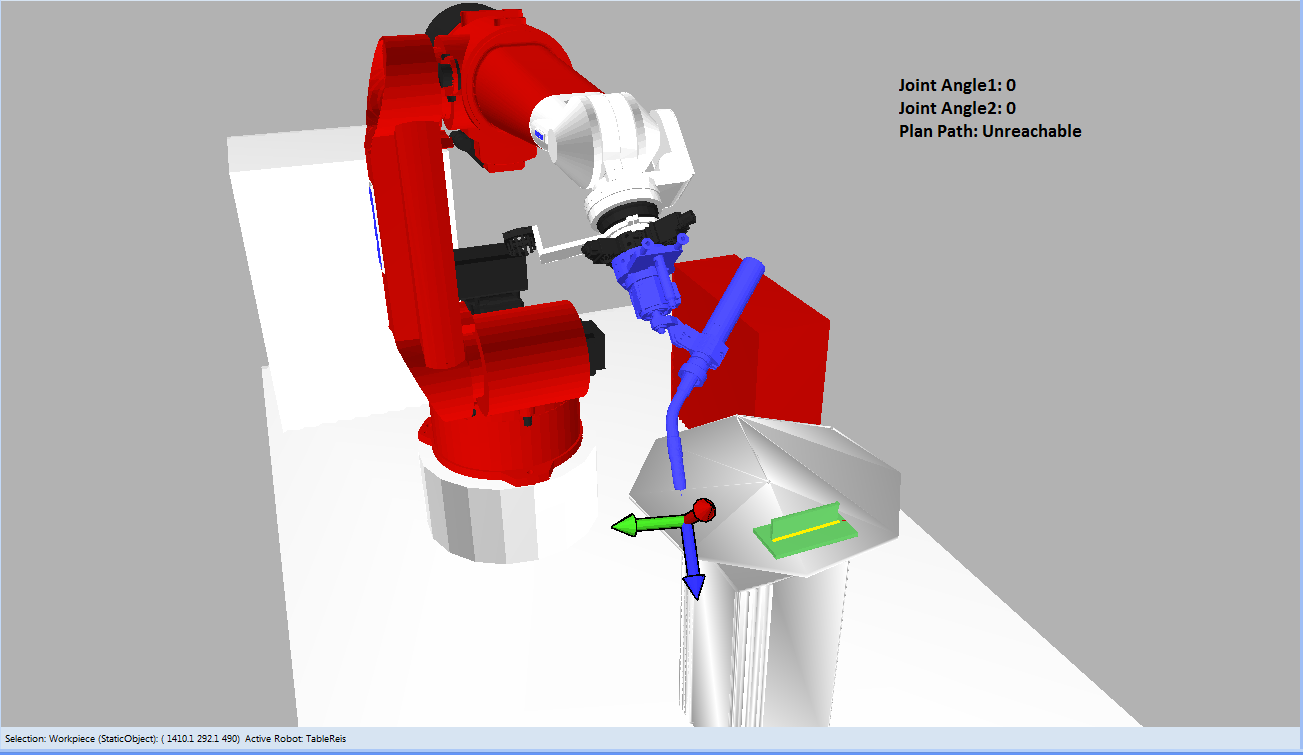
\includegraphics[width=0.8\textwidth,scale=0.6]{images/Urchbl_uscs.png}}
	\caption{Unreachable Use Case}
	\label{fig:rc1}
\end{figure} 
When an

\begin{figure}[!ht] %  figure placement: here, top, bottom, or page
	\centering
	\frame{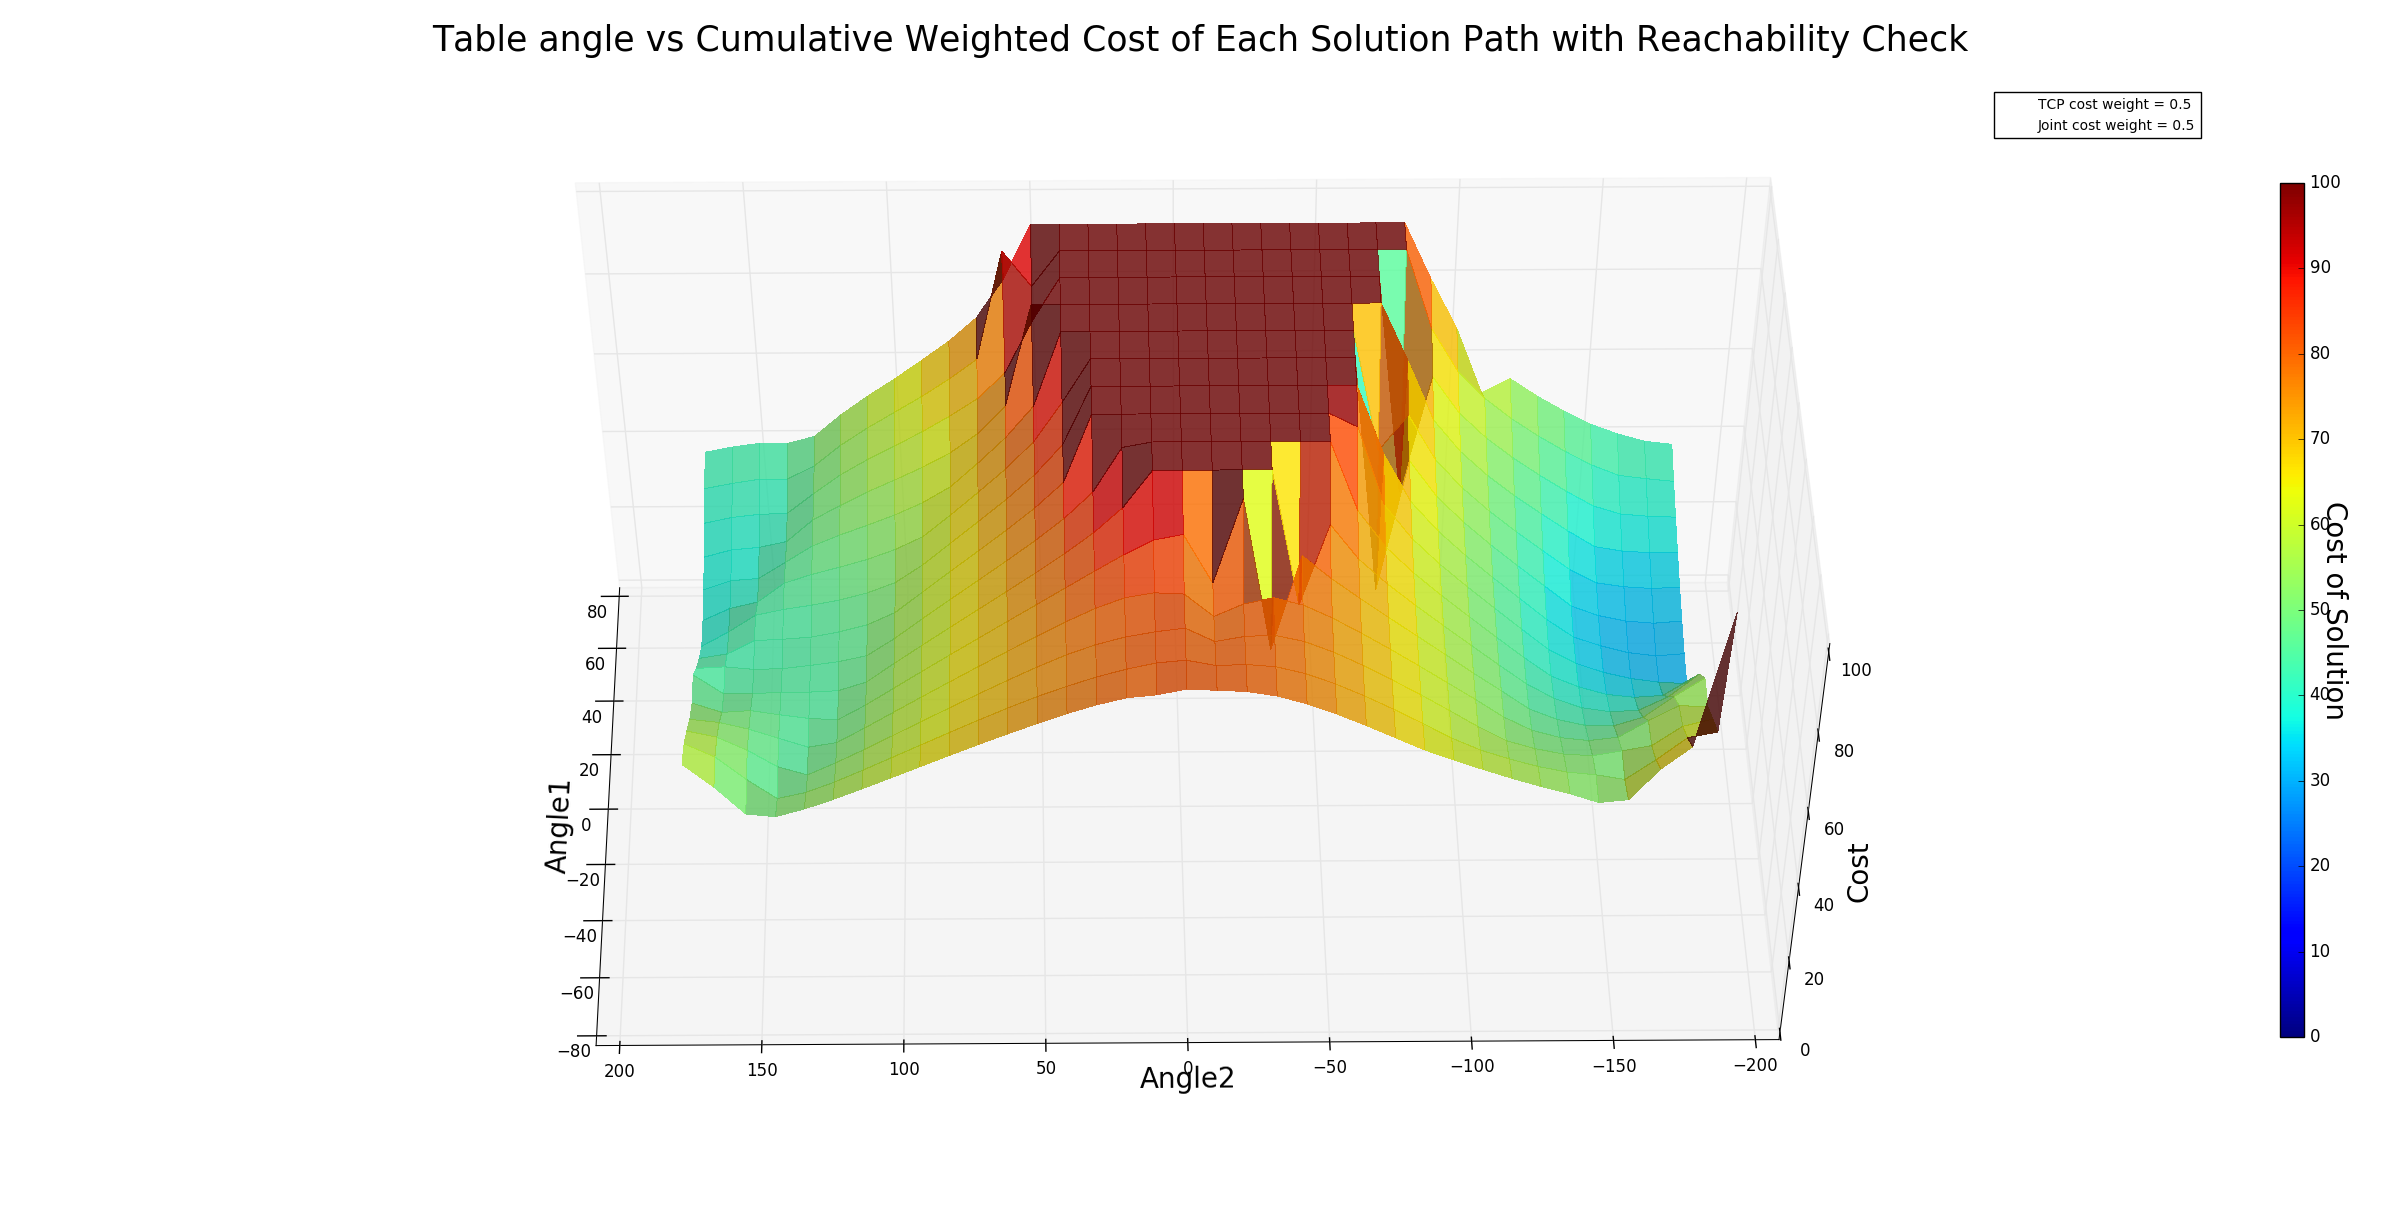
\includegraphics[width=0.8\textwidth,scale=0.6]{images/Rchbl_cst1.png}}
	\caption{Cost Space Plot}
	\label{fig:rc2}
\end{figure}

In figure \ref{fig:rc2}, the part marked with the deepest red color has the highest cost, i.e. weld paths generated for those joint angles of the table are unreachable. When joint angle 2 value either reaches $-180^{circle}$ or $+180^{circle}$ the cost value reaches its minimum. This can be explained by the fact that when joint angle 2 of the table rotates to either values, the selected workpiece edge faces the robot, thereby decreasing joint angle movement required by the manipulator for tracing the planned path. Facing the workpiece edge towards the manipulator also allows the tool tip orientation to follow the optimal orientation definition. 

A map for the reachable workspace of the manipulator, based on the table movement is presented in figure . Here we plot all the reachable weld plan path points. The points marked in magenta are unreachable, while the blue ones are reachable. 
\begin{figure}[!ht] %  figure placement: here, top, bottom, or page
	\centering
	\frame{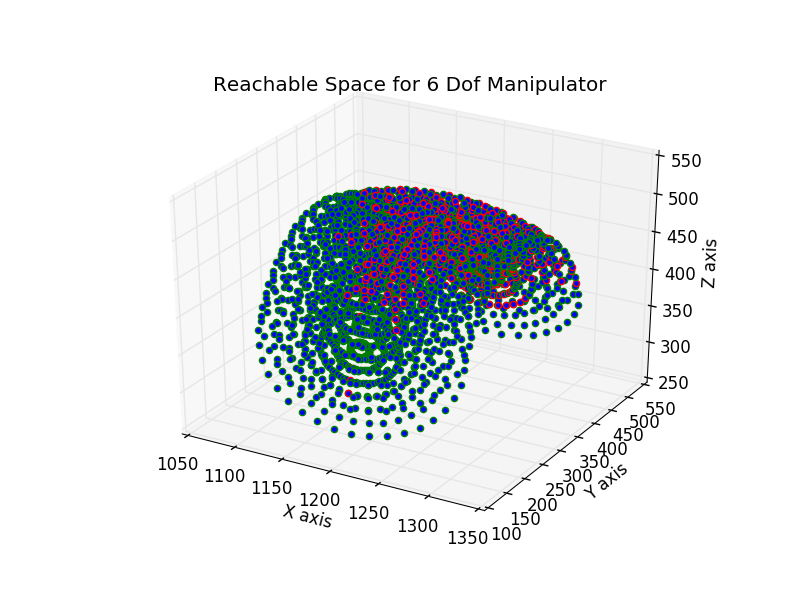
\includegraphics[width=0.8\textwidth,scale=0.6]{images/Rchbl_spc5.png}}
	\caption{Reachability Space Map}
	\label{fig:rc3}
\end{figure}

\subsection{Implementation and Results}
In the previous section \ref{ssec:usc1} we formulated the problem of unreachability into a cost function, in which the unreachable states were assigned high costs. Next, we use the approach described in section \ref{sssec:sa} in order to not only reposition the workpiece into a reachable position relative to the manipulator, but also ensure that it is in the most optimal position. The plot for the solution on the cost surface is illustrated in figure \ref{fig:rc4}. The start point is marked by the green '*' and the goal is marked by '+' sign. From the plot we can clearly observe that the algorithm reaches the global minima. 
\begin{figure}[!ht] %  figure placement: here, top, bottom, or page
	\centering
	\frame{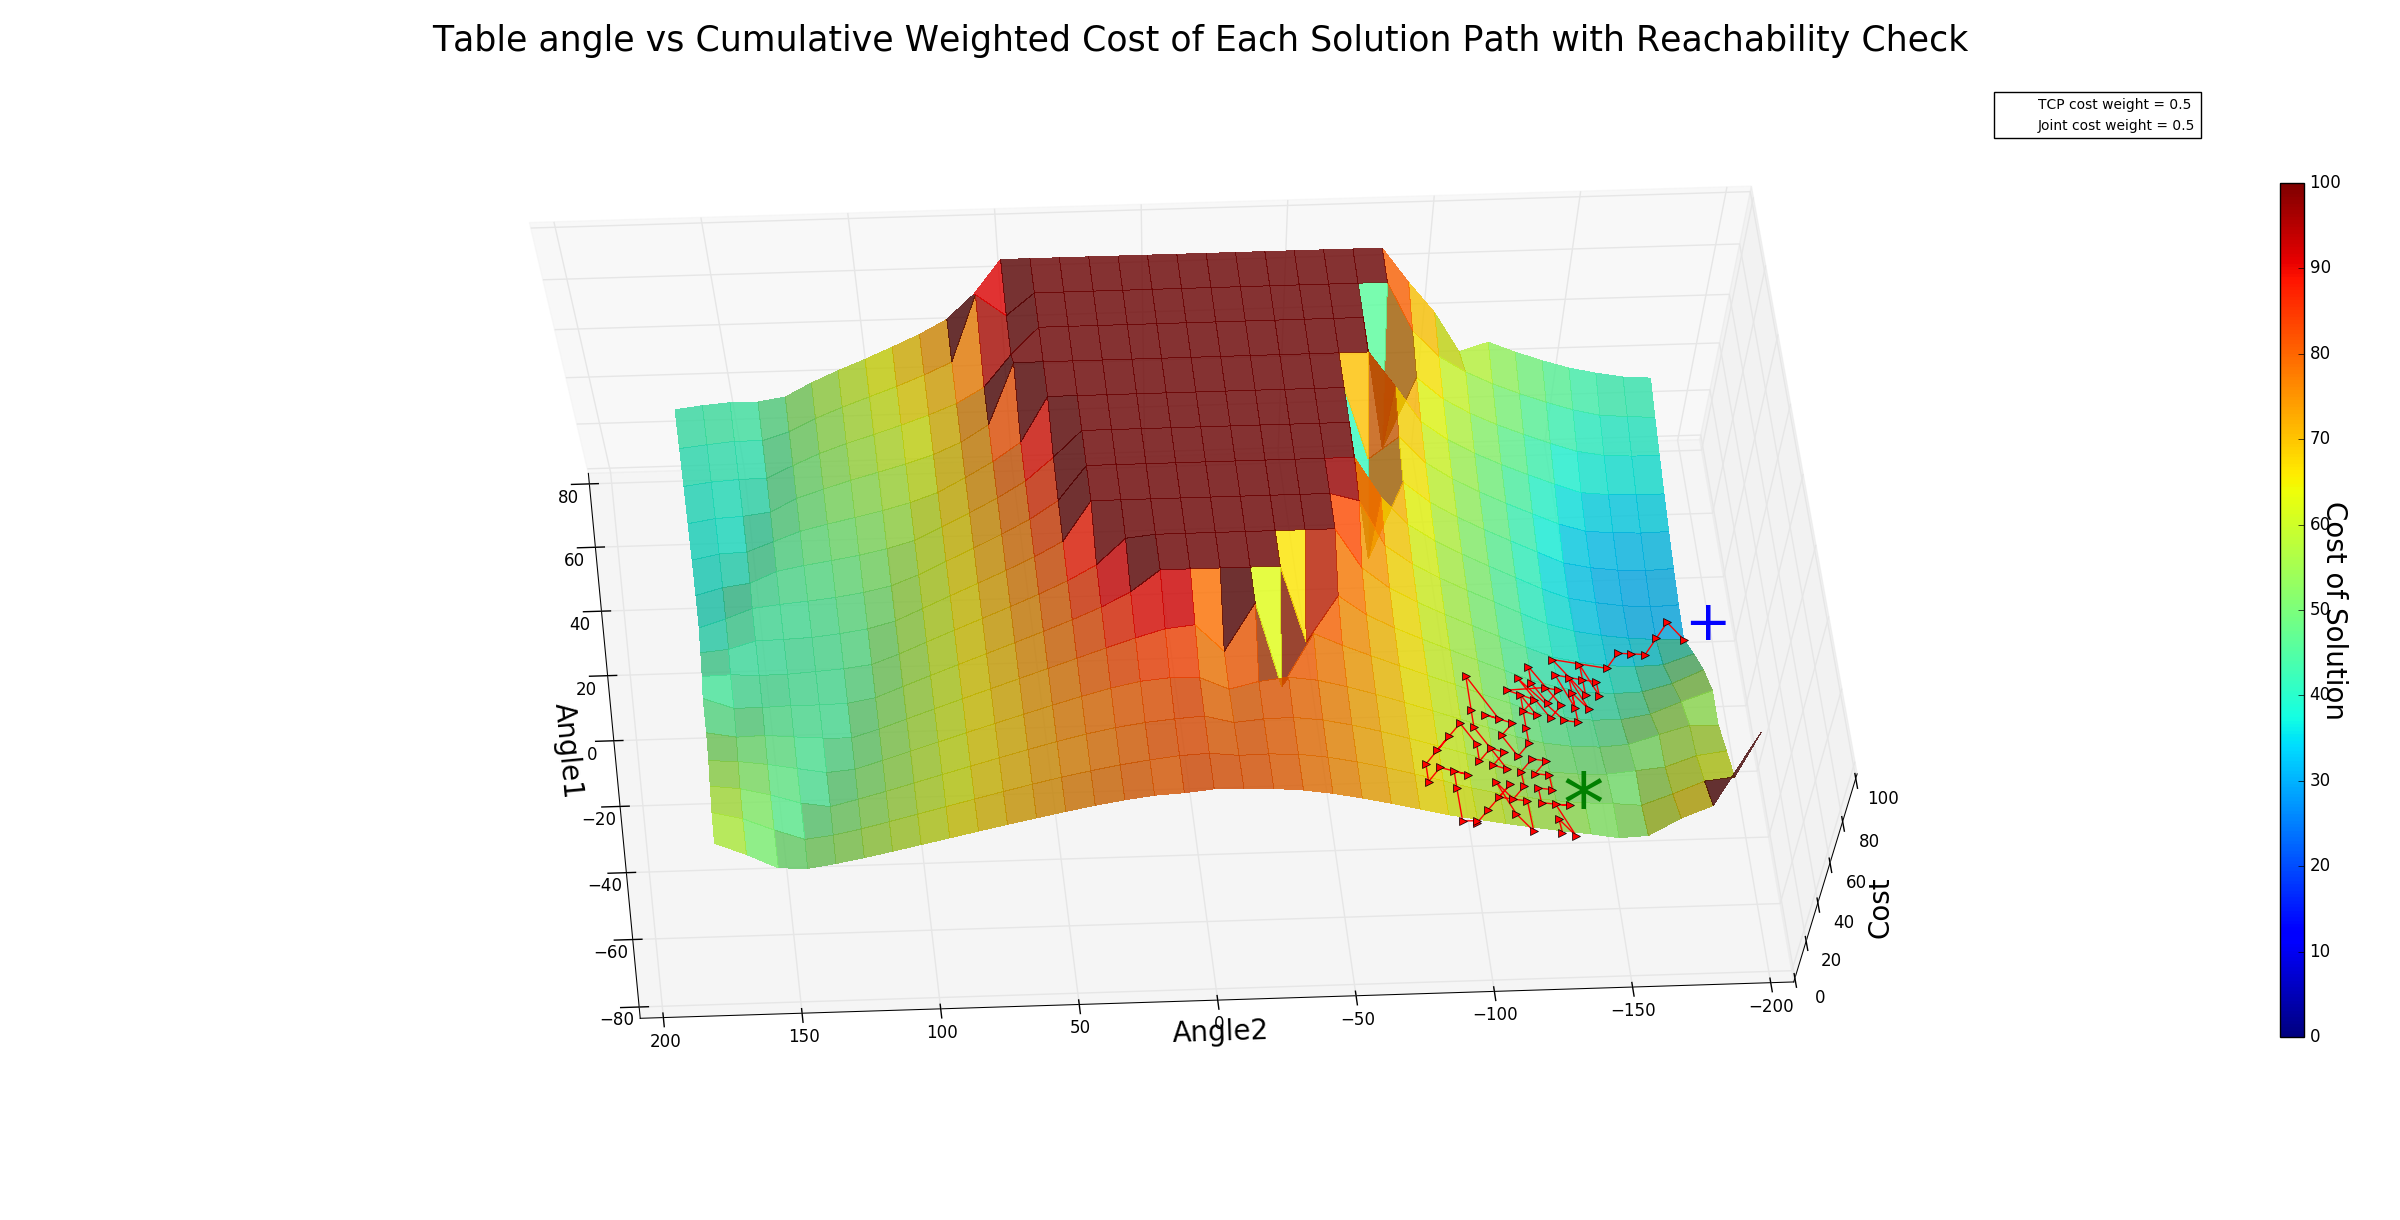
\includegraphics[width=0.8\textwidth,scale=0.6]{images/Rchbl_cst_sln.png}}
	\caption{Cost Plot of Reachability and Solution }
	\label{fig:rc4}
\end{figure}
The solution in RobotKit is shown in figure \ref{fig:rc5}.
\begin{figure}[!ht] %  figure placement: here, top, bottom, or page
	\centering
	\frame{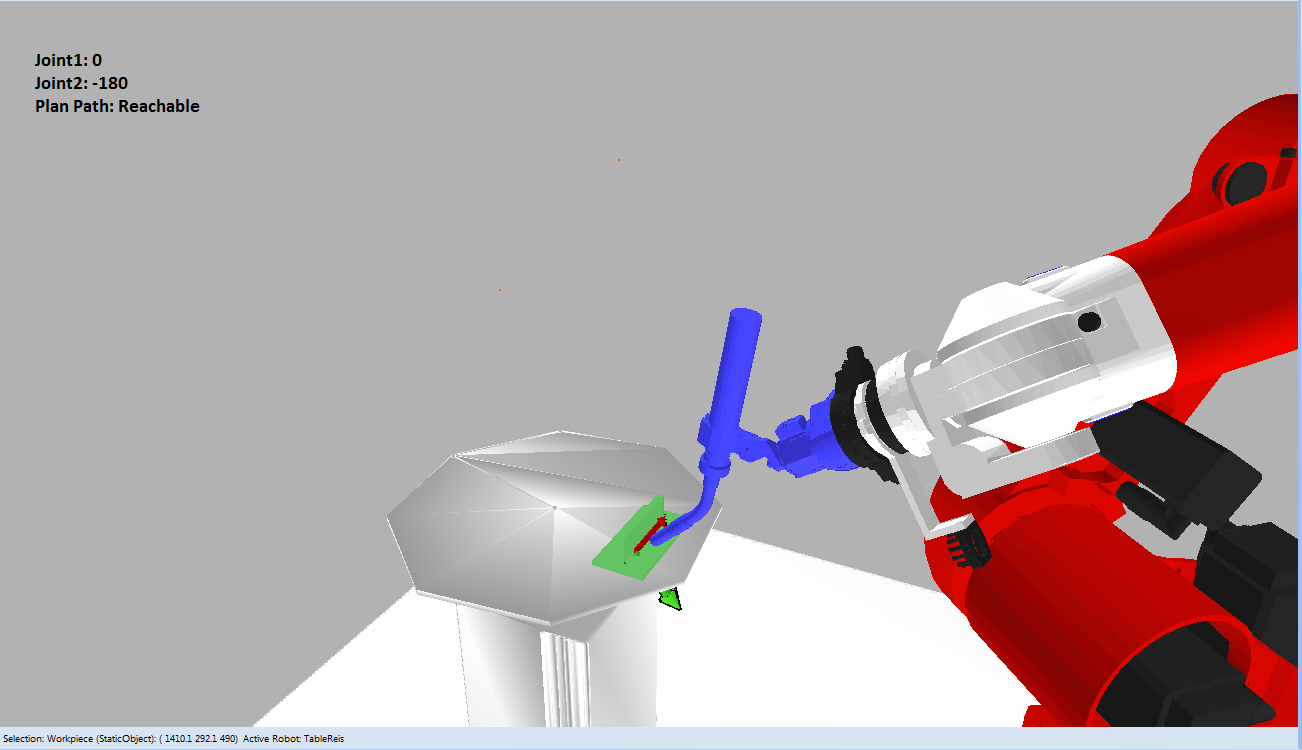
\includegraphics[width=0.8\textwidth,scale=0.6]{images/Urchbl_uscs_slv.png}}
	\caption{Cost Plot of Reachability and Solution }
	\label{fig:rc5}
\end{figure}
\clearpage


